%========== Balanced Binary Search Trees ==========%

\chapter{Balanced Binary Search Trees}
\label{ch:balancedbinarysearchtrees}

\textbf{Pensum} 12 + 13 \cite{clrs} \\\\
\textbf{Relevant Assignment} 13-3 \\\\
\textbf{Algorithms} Red-black tree, AVL-tree \\\\
\textbf{Keywords} ADT, BST structure- and property, rebalance, rotation
\vspace{1in}

\noindent A binary search tree is a node-based data structure that uses
pointers to keep the structure of a a set of nodes intact. Since the data
structure is purely held together by pointers, performing alterations on it
is very fast.
\\\\
\noindent \textbf{Structure} \\
Each node holds a $key$ and three pointers; one for each child-node, $left$
and $right$, and one for its parent-node $p$.
\\\\
\noindent \textbf{Property} \\
Let $x$ be a node in a binary search tree. If $y$ is a node in the left
subtree of $x$, then $y.key \leq x.key$. If $y$ is a node in the right
subtree of $x$, then $y.key \geq x.key$.

\newpage
\section{Operations}
Here we give the common operations performed on binary search trees.

\subsection{Searching}
Given the structure of a binary search tree, searching for a particular entry
is at most $O(\lg n)$, assuming that the tree is balanced. Should the tree not
be balanced the worst-case scenario is that the tree only has left- or right-
hand side children, which then produces a list, and searching a list takes
linear time $O(n)$. More specifically it is $O(h)$, where $h$ is the height.

\subsection{Minimum and Maximum}
The minimum and maximum procedures are simply search queries that looks only
to the left or right, in the cases of minimum and maximum, respectively. As
such, their running-time is the same as that of searching, $O(h)$.

% \subsection{Predecessor}
% ...

% \subsection{Successor}
% ...

\subsection{Insertion}
Inserting a node into a binary search tree is quite simple; we search through
the tree as usual until we find the spot where the node belongs. Since
everything else in this procedure is done in constant time $\Theta(1)$, and
all we are really doing is searching through the tree then it follows from the
search procedure that the running-time must be $O(h)$.

\subsection{Deletion}
The procedure of deleting a note $z$ from a tree $T$ has 3 basic cases:

\begin{enumerate}
\item{If $z$ has no children, we simply delete the node.}
\item{If $z$ has 1 child we elevate this child to the postion of $z$.}
\item{If $z$ has 2 children, we find the successor $y$, as $z$'s right child.
We put $y$ in place of $z$ and make the left subtree of $z$ the new left
subtree of $y$. The subtree of $y$ is then used as the right subtree, and is
constructed recursively as stated in this case.}
\end{enumerate}

\subsection{Rotation}
There are two forms of rotation; left- and right-rotation. These are simply
pointer manipulations of the immediate nodes.
\begin{figure}[H]
	\center
	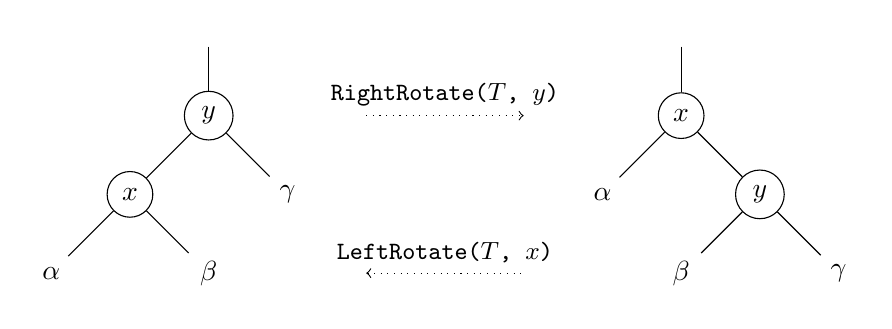
\begin{tikzpicture}
	[
	scale=1.0,
	align=center,
	empty/.style={},
	node/.style={circle, fill=white, draw=black},
	leaf/.style={circle, fill=white}
	]
		% transition
		\draw [->, dotted] (4, 2) -- node [above] {\small \texttt{RightRotate($T$, $y$)}} (6, 2);
		\draw [<-, dotted] (4, 0) -- node [above] {\small \texttt{LeftRotate($T$, $x$)}} (6, 0);
		
		% left
		\node (le) [empty] at 	(2, 3) {};
		
		\node (ly) [node] at 	(2, 2) {$y$};
		\node (lx) [node] at	(1, 1) {$x$};
		
		\node (la) [leaf] at 	(0, 0) {$\alpha$};
		\node (lb) [leaf] at 	(2, 0) {$\beta$};
		\node (lc) [leaf] at 	(3, 1) {$\gamma$};
	
		% right
		\node (re) [empty] at 	(8, 3) {};
		
		\node (ry) [node] at 	(9, 1) {$y$};
		\node (rx) [node] at	(8, 2) {$x$};
		
		\node (ra) [leaf] at 	(7, 1) {$\alpha$};
		\node (rb) [leaf] at 	(8, 0) {$\beta$};
		\node (rc) [leaf] at 	(10, 0) {$\gamma$};	
		% drawing code
		\foreach \from/\to in {le/ly,ly/lx,lx/la,lx/lb,ly/lc} \draw (\from) -- (\to);
		\foreach \from/\to in {re/rx,rx/ra,rx/ry,ry/rb,ry/rc} \draw (\from) -- (\to);
	\end{tikzpicture}
	\caption{Left- and right BST rotations}
	\label{fig:bst-rotations}
\end{figure}
Since all we are doing is to change a few pointers, the procedure takes
constant time $\Theta(1)$.

% \section{Rebalancing}
% When we use a balanced implementation of binary search trees, such as
% \textit{red-black}- or \textit{AVL}-trees, we must maintain certain
% properties, which are typically accounted for after applying an alteration on
% the tree - this is called \textit{rebalancing} - whenever a tree gets
% unbalanced, as the result of an operation performed on it, we say that the
% tree is \textit{left- or right heavy}.

\section{Red-Black Binary Search Tree}
A red-black BST is a implementation of balanced binary search trees, and it
works by figuratively coloring each node in the tree one of two colors; red or
black. By the use of constraints on these colorings, and taking action
whenever we have a violation of the constraints, we can ensure that the tree
remains balanced --- hence also a minimum tree height, which in turn, also
gives us good performance.

\subsection{Properties}
These are the properties of red-back binary search trees.
\begin{enumerate}
	\item Every node is either red or black.
	\item The root is black.
	\item All leaves (\texttt{NIL}) are black.
	\item Both children of red nodes are black.
	\item All simple paths from a node to descendants leaves contain the same
number of black nodes.
\end{enumerate}
For red-black trees we define the \textit{black height} as the number of black
nodes on any simple path from, but not including, a node $x$ down to a leaf
--- we denote this as $\textnormal{bh}(x)$. This follows from property 5. We
define the black height of a red-black tree to be the black height of its
root.

\subsection{Analysis}
We claim that red-black trees are balanced and thus guarantees a running-time
of $O(\lg n$. This follows from lemma 13.1\cite[p. 309]{clrs}, which states
\\\\
\noindent \textbf{Claim}
A red-black tree with $n$ internal nodes has height at most $2\lg(n+1)$.

\begin{lemma} {\ }\\
	Let $s(x)$ denote the number of internal nodes in a subtree rooted at any
	node $x$, then
	\begin{align}
		s(x) \geq 2^{\textnormal{bh}(x)} - 1
	\end{align}
\end{lemma}

\begin{proof}[Proof of claim]
	\begin{align}
		n = s(r) \geq 2^{\textnormal{bh}(r)} - 1 \geq 2^{h/2} - 1
	\end{align}
	By property 4 it follows that at least half of the nodes on any simple
	path from the root to a leaf, excluding the root, must be a black.
	\begin{align}
		n + 1 \geq 2^{h/2} \Leftrightarrow
		\lg(n+1) \geq \frac{h}{2} \Leftrightarrow
		2 \lg(n+1) \geq h
	\end{align}
\end{proof}

\begin{proof}[Proof of lemma] {\ } \\\\
	\textbf{Base case} \\
	Valid when $x$ has height $0$; $x$ is an external leaf, and $s(x) = 0$,
	thereby $\textnormal{bh}(x) = 0$ and $2^{\textnormal{bh}(x)}-1 = 0$, so
	the inequality holds.
	\\\\
	\textbf{Inductive step} \\
	Assume that the inequality holds for all nodes of height less than $k$ and
	let $x$ be a node with $\textnormal{h}(x) = k$, and let
	$\textnormal{L}(y)$ and $\textnormal{R}(y)$ denote the left and right
	subtrees of a node $y$, respectively.
	
	\begin{align}
		\textnormal{h}(L(x)) \leq k-1
		\quad \text{and} \quad
		\textnormal{h}(R(x)) \leq k-1
	\end{align}
	$\therefore$ lemma is valid for $\textnormal{L}(x)$ and $\textnormal{R}(x)$.
	
	\begin{align}
		s(x) &= s(\textnormal{L}(x)) + s(\textnormal{R}(x)) + 1 \\
		&\geq 2^{\textnormal{bh}(\textnormal{L}(x))}-1
		+ 2^{\textnormal{bh}(\textnormal{R}(x))}-1 + 1 \\
		&= 2^{\textnormal{bh}(x-1)}-1 + 2^{\textnormal{bh}(x-1)}-1 + 1 \\
		&= 2^{\textnormal{bh}(x-1)} + 2^{\textnormal{bh}(x-1)}-1 \\
		&= 2^{\textnormal{bh}(x)}-1
	\end{align}
	Hence, the height falls by at most 1.
\end{proof}
The immediate consequence of this, is that the common operations on binary
search trees runs in $O(\lg n)$ with a red-black balanced implementation of
the operations that alter the tree, such as insertion and deletion.

